\documentclass[a4paper,11pt]{article}
\usepackage[utf8]{inputenc}
\usepackage[paper=a4paper, hmargin=1.5cm, bottom=1.5cm, top=3.5cm]{geometry}
\usepackage[T1]{fontenc}
\usepackage[spanish]{babel}
\usepackage[colorlinks=true, linkcolor=blue]{hyperref} %Links para el indice.
\usepackage{amsfonts}
\usepackage{graphicx}
\usepackage{float}
\usepackage{verbatim}
\usepackage{listings}
\usepackage{algorithm}
\usepackage{algpseudocode}
\usepackage{graphicx}
\usepackage{caption}
\usepackage{subcaption}

\usepackage[section]{placeins}
\usepackage{float}
\usepackage{amsmath}
\usepackage{blindtext}
\usepackage{sidecap}
\usepackage{color}

\newcommand{\real}{\hbox{\bf R}}

\title{Trabajo Práctico de Métodos Númericos}
\author{Castro, Dami\'an \& Matayoshi, Leandro \& Szyrej,Alexander}

\begin{document}

\begin{center}
	Universidad de Buenos Aires - Departamento de Computaci\'on - FCEN
\end{center}

\rule{\linewidth}{0.5mm}

\vspace{1cm}

\begin{center}
	\Huge{Trabajo Práctico de Métodos Númericos}
\end{center}


\vspace{4cm}


Integrantes:
\begin{itemize}
	\item Castro, Dami\'an L.U.: 326/11  \verb+ltdicai@gmail.com+
	\item Matayoshi, Leandro L.U.: 79/11 \verb+leandro.matayoshi@gmail.com+
	\item Szyrej, Alexander L.U.: 642/11   \verb+alexanderszyrej@gmail.com+
	
\end{itemize}


\maketitle

\vspace{4cm}

Palabras Clave:
%\begin{itemize}
	
%\end{itemize}



\newpage

\tableofcontents

\newpage

\section{Introducción teórica}

%	En este trabajo práctico se nos pidió analizar el comportamiento de un modelo de una estructura conocida como 
puente Pratt Truss al simular la aplicación de peso sobre el mismo.
	El modelo consiste en una representación en 2 dimensiones del puente. Llamamos \emph{span} al largo de la base 
y \emph{h} a la altura del mismo. A su vez cuenta con una cantidad par \emph{n} de secciones, $2*n$
juntas, $4*n-3$ links y 3 fuerzas adicionales que actúan sobre el puente, a las que llamamos $h_{0}$, $v_{0}$ y
$v_{1}$.
	A su vez, en las $(n-1)$ juntas inferiores centrales es posible insertar cargas que representan el peso 
ejercido sobre dichas juntas.
	Este modelo nos permite analizar la evolución del sistema al alterar cada uno de los distintos factores,
como el \emph{span}, la altura y el peso de las cargas.
	Concretamente el objetivo fue diseñar un algoritmo que, dada una instancia de puente Pratt Truss con una configuración de
cargas iniciales calcule el valor de las fuerzas ejercidas sobre cada uno de los links.
	Para ello planteamos un sistema de ecuaciones (la deducción del mismo aparece explicada en el desarrollo) y
establecemos una equivalencia entre resolver el problema y hallar la solución de $Ax = b$.

1) $A$ representa la forma en que interactúan los links sobre cada una de las juntas. Cada una de las filas de la matriz 
representa una ecuación de fuerzas que actúan sobre la junta (una para el plano vertical y otra para el horizontal). Sabemos
que las fuerzas actuantes en cada plano para cada junta deben estar en equilibrio.

2) \emph{x} es el vector de $4n$ fuerzas que constituyen las incógnitas de nuestro problema.

3) \emph{b} es un vector de $4n$ valores. Estas fuerzas intervienen en las ecuaciones mencionadas en el punto (1). Las fuerzas
actuantes en cada plano para cada junta deben estar en equilibrio (Es decir, la suma de las mismas debe ser igual a 0). Las
cargas forman parte de este vector (actúan sobre el plano vertical). Los valores de \emph{b} para las ecuaciones
correspondientes al plano horizontal son iguales a 0.

Es posible demostrar que la matriz \emph{A} cumple la propiedad de ser banda $p,(q+p)$. Por lo tanto utilizamos en nuestros
algoritmos una representación que nos permite ganar eficiencia en cuestiones de tiempo y espacio.
El método seleccionado para resolver el problema fue Eliminación Gaussiana con pivoteo parcial. Una buena explicación del
mismo puede ser encontrada en el libro ''Numerical analysis'',\emph{Burden, Faires}. El método implementado está adaptado
a la representación de la matriz elegida.

	La última parte del trabajo consistió en desarrollar un método heurístico para aplicar en los casos donde el 
máximo de los módulos de las fuerzas halladas supere cierto valor (parámetro de entrada). La idea es
modificar la estructura insertando pilares (y de esta manera generando subestructuras)
para tratar de reducir la magnitud de las fuerzas ejercidas sobre los links, aunque evitando insertar pilares innecesarios
ya que los mismos son costosos. Una heurística es un algoritmo que, si bien no necesariamente encuentra la solución óptima
a nuestro problema (por ejemplo, porque esto podría ser muy costoso) propone una solución aceptable.


\section{Desarrollo}

%\input{desarrollo1.tex}
Hemos probado entonces que nuestra matriz es banda 3,4. Sin embargo durante la aplicación 
de eliminación Gaussiana con pivoteo parcial eventualmente será necesario realizar intercambio de filas. 
Demostremos que luego de aplicar este método sobre una matriz banda $b_{p,q}$, la matriz resultante es banda $b_{p,(p+q)}$


\subsection{Demostración por inducción sobre el i-ésimo paso de la eliminación Gaussiana}

~

Sea $b_{p,q} \in R^{nxn}$, y sea $b^{i}$ la matriz resultante luego de aplicar el i-ésimo paso de eliminación Gaussiana con
pivoteo parcial. Probemos que al finalizar el método, la matriz $b^{n-1}$ obtenida es banda p, q+p.

~

\subsubsection{Caso base}

~

En el primer paso del método pueden suceder 2 cosas:

1) No se produce pivoteo sobre la primera fila $\Rightarrow$ demostración es trivial.

2) Se produce el intercambio entre la fila 1 y una fila $j$ con $1<j \leq (p+1)$. 

~

\underline{Bandas en la fila j al intercambiar fila 1 con fila j:}

La banda izquierda está determinada por la diferencia entre $j$ y la columna de menor índice que contenga un elemento distinto
de cero: llamemos a este índice $i$. Notemos que en el peor caso $i=1$ $\Rightarrow$ Banda izquierda = $j-i \leq (p+1) - i \leq
(p+1) - 1 = p$. (El máximo ancho de banda ''izquierda'' se produce al intercambiar la primera fila con la $p+1$.)

La banda derecha está determinada por la diferencia entre la columna de mayor índice $k$
que contenga un elemento distinto de cero y $j$ . Notemos que en el peor caso $j=2$ y $k =1+q$ $\Rightarrow$ Banda derecha =
$k-j \leq (1+q) -2 = (q-1)$. (El máximo ancho de banda ''derecha'' se produce al intercambiar la primera fila
con la segunda)

Por lo tanto la fila $j$ (en cualquiera de los casos) mantiene la propiedad de ser banda p,(p+q).

~

\underline{Bandas en la fila 1 al intercambiar fila 1 con fila j:}

Como estamos analizando la primera fila, es inmediato ver que la banda izquierda continúa siendo $p$, ya que no hay elementos
a la izquierda de la columna 1.

La banda derecha está determinada por la diferencia entre la columna de mayor índice $k$ que contenga un elemento distinto
de cero y la columna 1. Notemos que en el peor caso $j=1+p$ y $k=j+q$ $\Rightarrow k-1 = 1+p+q-1 = p+q$. (El máximo ancho de 
banda ''derecha'' se produce al intercambiar la primera fila con la $p+1$.)

Por lo tanto, la primera fila mantiene la propiedad de ser banda p,(p+q).

~

Sea $k$ una fila tal que $1 \leq k \leq (p+1)$. Luego de realizar el primer paso de Gauss y generar los ceros en la 
primera columna tenemos que:

- Banda izquierda de k $\leq (k-1) \leq (p+1)-1 = p$

- Banda derecha de k $ \leq (1+p+q)-k \leq p+q $

Como el resto de las filas no han sido modificadas, podemos afirmar que $b^{1}$ es banda p,(p+q). 
Demostrado caso base $\square$

~

\subsubsection{Paso inductivo: $P(i-1) \Rightarrow P(i)$}

~

Sea $j$ tal que $0 \leq j \leq (p-1)$. Analicemos brevemente qué sucede con cada una de las filas $i+j$.
En la matriz inicial $b^{0}$ sabíamos que el elemento más a la derecha para cada una de ellas estaba a lo sumo en la columna:
$i+j+q$. Sin embargo esta situación pudo haber cambiado luego de realizar el paso (i-1)-ésimo. En esta instancia, el
elemento más a la derecha podría estar a lo sumo en la columna: $i+p+q-1$. Notemos que $i+j+q \leq i+p+q-1 , \ \forall 
\ 0 \leq j \leq (p-1)$.

\begin{figure}[!h]
	\begin{center}
		  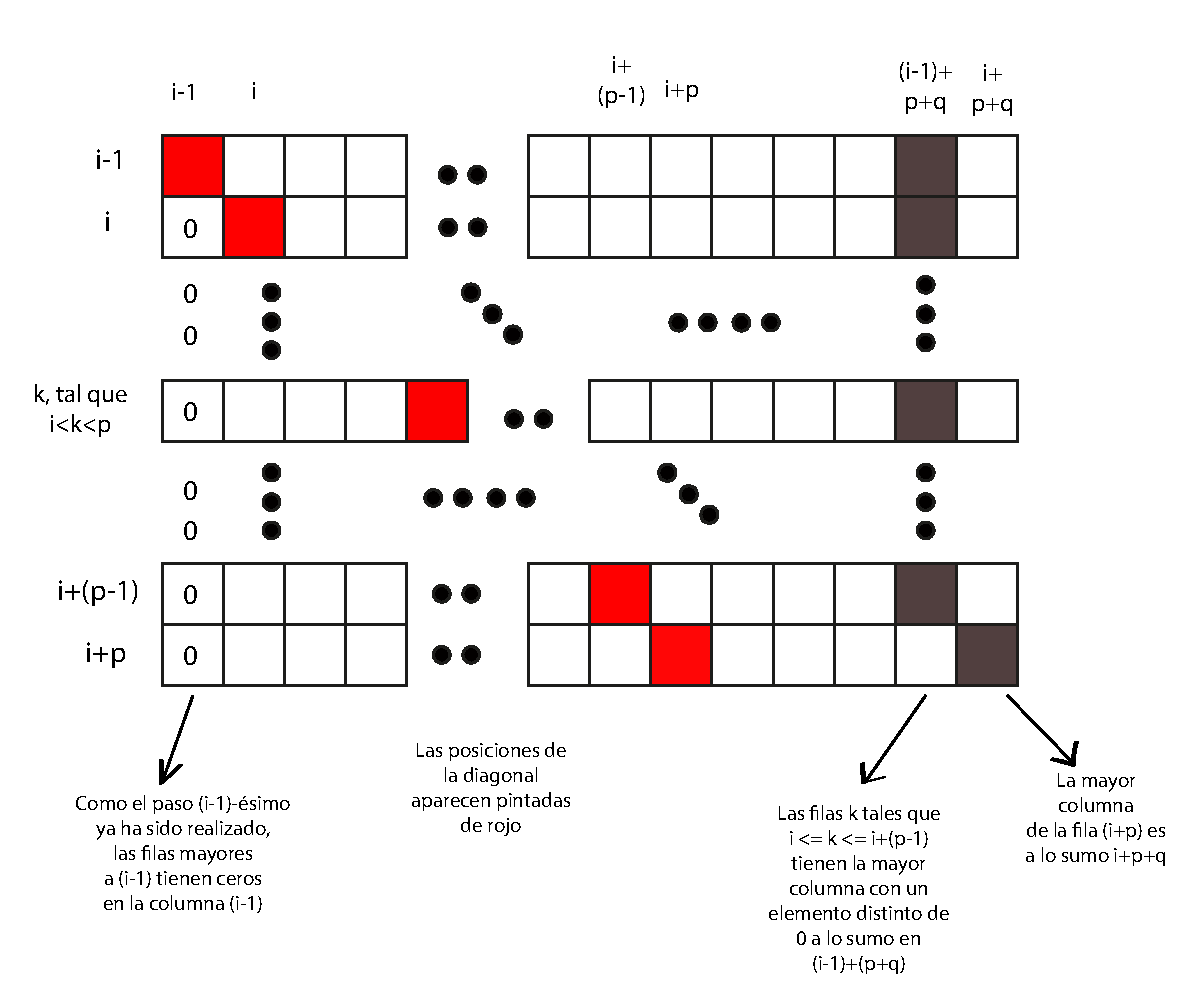
\includegraphics[scale=0.5]{Imagenes/im_8.pdf}
		  \caption{Estado de la matriz luego de realizar el (i-1)-ésimo paso. Se muestran únicamente
		  las filas y columnas que intervienen en el i-ésimo paso}
		  \label{fig:contra1}
	\end{center}
\end{figure}
\FloatBarrier

Para la fila $(i+p)$ la columna de mayor índice es a lo sumo $(i+p+q)$. Es suficiente probar que la matriz se mantiene como 
banda (p,p+q) luego de intercambiar las filas $i$ e $i+p$ ya que constituye el peor caso que podría ensanchar las bandas.

\begin{figure}[!h]
	\begin{center}
		  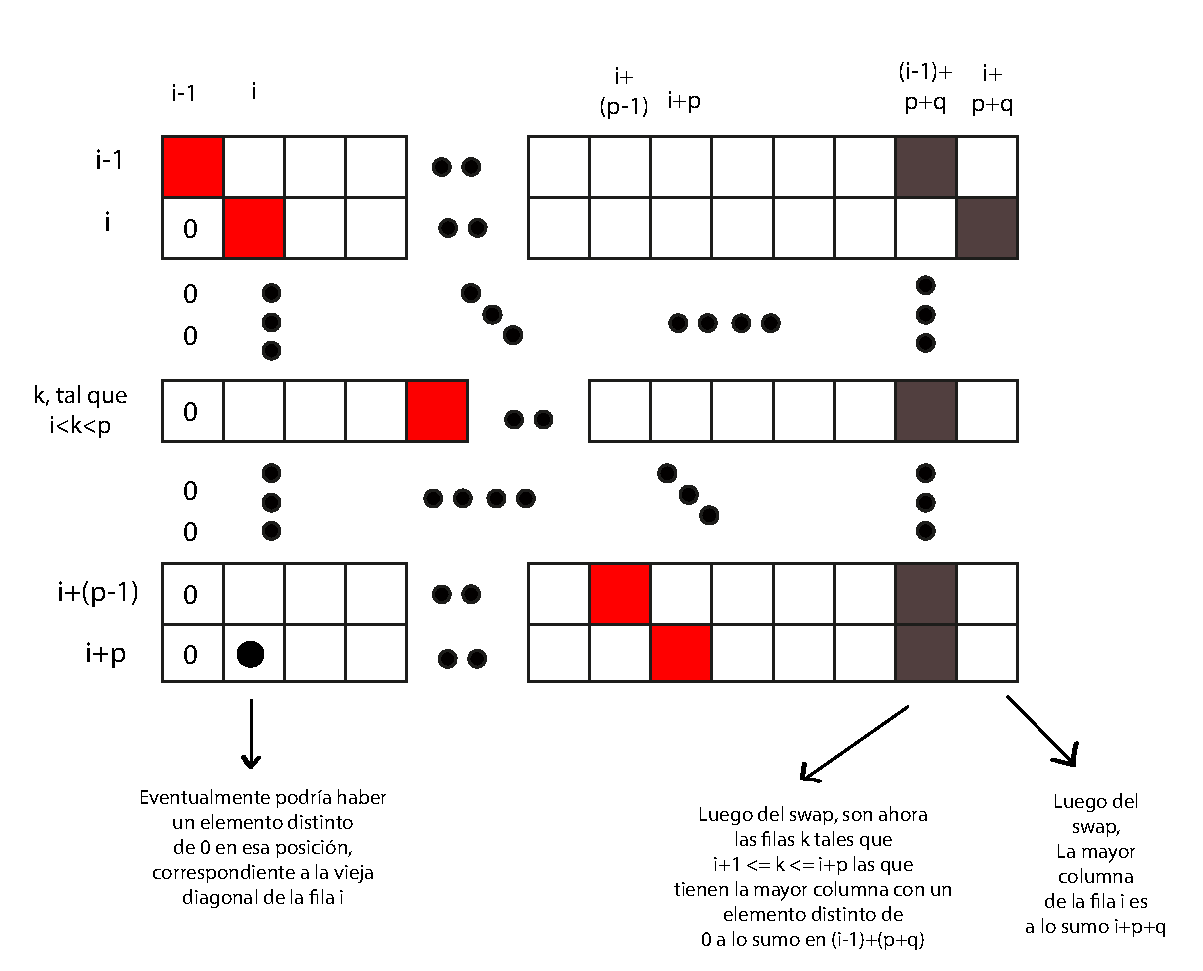
\includegraphics[scale=0.5]{Imagenes/im_9.pdf}
		  \caption{$b^{(i-1)}$ al swapear las filas i e (i+p), ya que constituye el peor caso que podría ensanchar
		  las bandas.}
		  \label{fig:contra1}
	\end{center}
\end{figure}

~

\underline{Bandas en la fila $i$ al intercambiar fila $i$ con fila $i+p$}

$Banda \ izquierda \leq i - (i+p-p) = 0$ (Columna de la diagonal menos columna del elemento más a la izquierda)

$Banda \ derecha \leq (i+p+q) - i = p+q$ (Columna del elemento más a la derecha menos columna diagonal)

La fila $i$ mantiene la propiedad de ser banda p,(p+q).

~

\underline{Bandas en la fila $i+p$ al intercambiar fila $i$ con fila $i+p$}

Como ya se han puesto ceros en las columnas a la izquierda de la i-ésima, tenemos que:

$Banda \ izquierda \leq (i+p) - (p) = 0$ (Columna de la diagonal menos columna del elemento más a la izquierda)

$Banda \ derecha \leq (i+p+q-1) - (i+p) \leq p+q$ (Columna del elemento más a la derecha menos columna diagonal)

La fila $(i+p)$ mantiene la propiedad de ser banda p,(p+q).

~

\begin{figure}[!h]
	\begin{center}
		  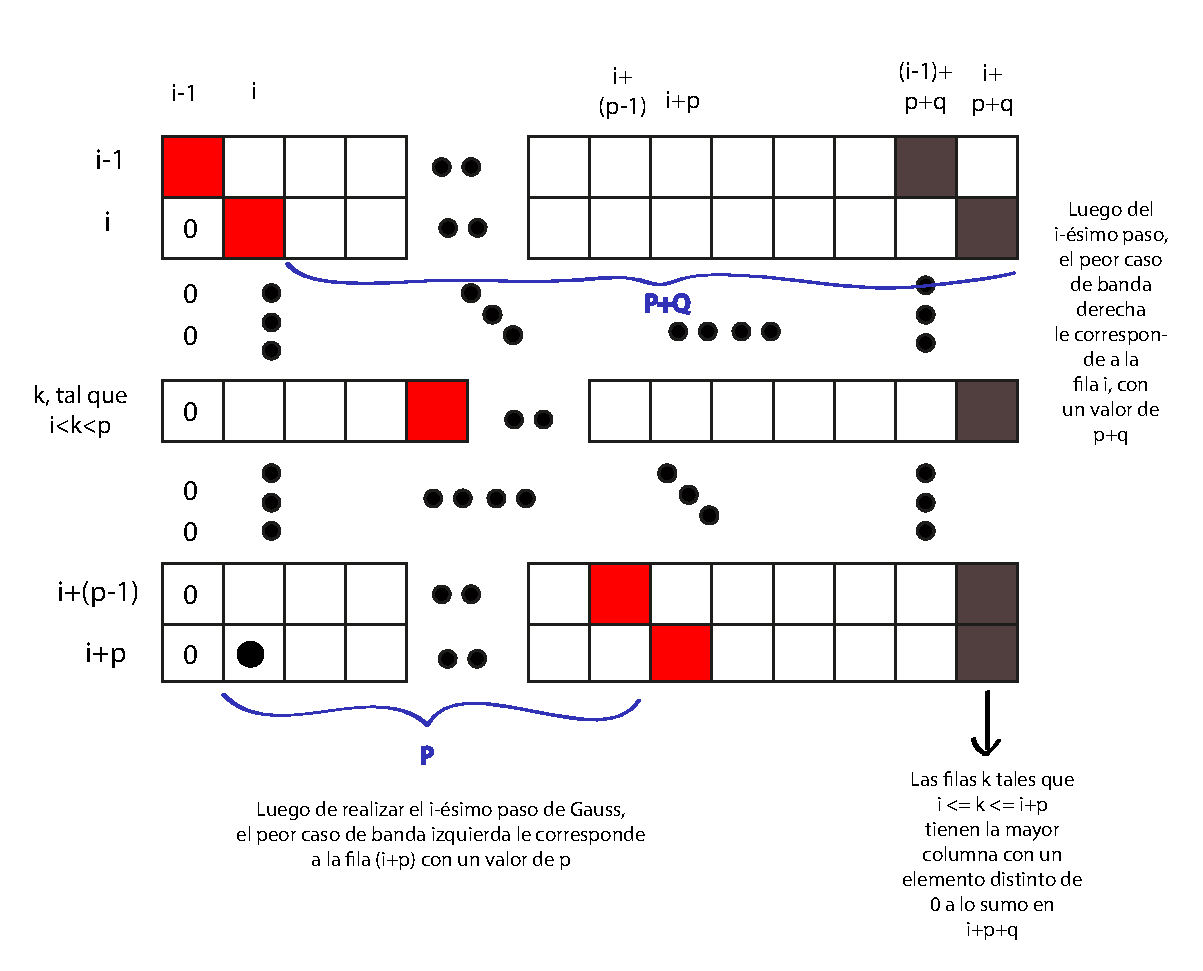
\includegraphics[scale=0.5]{Imagenes/im_10.pdf}
		  \caption{$b^{(i)}$ al realizar el paso habiendo intercambiado las filas i e (i+p)}
		  \label{fig:contra1}
	\end{center}
\end{figure}

Sea $k$ una fila tal que $i \leq k \leq (i+p)$. Luego de realizar el i-ésimo paso de Gauss y generar los ceros en la 
i-ésima columna tenemos que:

- Banda izquierda de k $\leq (k-i) \leq (i+p)-i = p$

- Banda derecha de k $ \leq (i+p+q)-k \leq (i+p+q)-i = p+q $

Como el resto de las filas no han sido modificadas, podemos afirmar que $b^{i}$ es banda p,(p+q). 
Demostrado paso inductivo $\square$



\section{Resultados y discusión}

%Tal como mencionamos en el desarrollo, la experimentación fue realizada para valores de $n= 4,6,8,10,12,16,32,64,128$. Entre 
ellos, fueron seleccionados los resultados más representativos y en donde creemos que se observa
mejor aquello que queremos mostrar.

\subsection{Variando el span}

Para este experimento, dado $n$, fijamos el valor de $h=n$, el valor de las cargas $c_{i}=1 \ \forall i$, y fuimos aumentando el
valor del \emph{span} en múltiplos de $n$, calculando en cada caso el valor de la máxima fuerza en módulo. Es decir, en primer lugar
$span=1*n$, luego $span=2*n$, \ldots.

\begin{figure}[!h]
	\begin{center}
		  \includegraphics[scale=0.4]{Imagenes/variable_span/n_4}
		  \caption{Máxima fuerza en módulo en función de la longitud del span, para $n=4$}
		  \label{fig:contra1}
	\end{center}
\end{figure}
\FloatBarrier

\begin{figure}[!h]
	\begin{center}
		  \includegraphics[scale=0.4]{Imagenes/variable_span/n_8}
		  \caption{Máxima fuerza en módulo en función de la longitud del span, para $n=8$}
		  \label{fig:contra1}
	\end{center}
\end{figure}
\FloatBarrier

\begin{figure}[!h]
	\begin{center}
		  \includegraphics[scale=0.4]{Imagenes/variable_span/n_32}
		  \caption{Máxima fuerza en módulo en función de la longitud del span, para $n=32$}
		  \label{fig:contra1}
	\end{center}
\end{figure}
\FloatBarrier

Los resultados nos permiten corroborar nuestra primera hipótesis: El módulo de las fuerzas ejercidas sobre los links aumentan en función
del \emph{span}. Según lo que muestran los gráficos parecería ser que este aumento se da de forma directamente proporcional. Un hecho
importante que no estamos observando es que en los 3 experimentos, para cualquier valor de $n$, el link sobre el cual se ejerce 
la fuerza de módulo máximo es $2*n-1$. (Es algo razonable, teniendo en cuenta que el peso de las cargas está uniformemente 
distribuído).

~

\begin{figure}[!h]
	\begin{center}
		  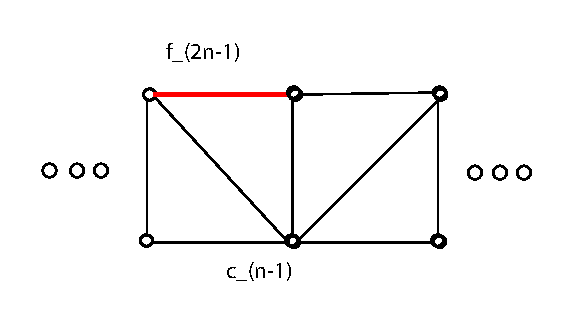
\includegraphics[scale=0.75]{Imagenes/im_12.pdf}
		  \caption{Fuerza $2*n-1$}
		  \label{fig:contra1}
	\end{center}
\end{figure}
\FloatBarrier

~

\subsection{Variando el valor de las cargas}

\subsubsection{Aumentando el peso de una única carga}

En primer lugar realizamos un experimento en donde únicamente variamos el valor de una de las cargas, manteniendo fijos el $span=n$
y $h=n$. En otras palabras, siendo $n$ la cantidad de secciones, generamos $\frac{n}{2}$ instancias distintas en donde el valor
de las cargas varía de la siguiente manera:

1) En la primera, peso de la carga aplicada sobre $c_{1}=100$ (primera junta inferior con carga)
. Peso de las cargas aplicadas sobre el resto de las juntas = 1.

2) En la segunda, peso de la carga aplicada sobre $c_{3}=100$ (segunda junta inferior con carga)
. Peso de las cargas aplicadas sobre el resto de las juntas = 1.

\ldots

n/2) En la $\frac{n}{2}$, peso de la carga aplicada sobre $c_{(n-1)}=100$. (junta inferior del medio con carga).
Peso de las cargas aplicadas sobre el resto de las juntas = 1.

~

A continuación se exhiben los resultados obtenidos para valores de $n=6,8,16$

\underline{Experimentación con $c_{1} = 100$}

\begin{center}
    \small{
    \begin{tabular}{| l | l | l | l | l | }
    \hline
    n & max\_fuerza($c_{1}=100$) & link más afectado & max\_fuerza($c_{1}=0$) & link más afectado\\ \hline 
    6 & 120.208 & 3 & 4 & 11 \\ \hline
    8 & 127.456 & 3 & 7.5 & 15 \\ \hline
    16 & 141.863 & 3 & 31.5 & 31 \\ \hline
    \end{tabular}
    }
\end{center}

~

\underline{Experimentación con $c_{3} = 100$}

\begin{center}
    \small{
    \begin{tabular}{| l | l | l | l | l | }
    \hline
    n & max\_fuerza($c_{3}=100$) & link más afectado & max\_fuerza($c_{3}=0$) & link más afectado\\ \hline 
    6 & 136 & 7 & 3.5 & 11 \\ \hline
    8 & 154.5 & 7 & 7 & 15 \\ \hline
    16 & 187.25 & 7 & 31 & 31 \\ \hline
    \end{tabular}
    }
\end{center}

~

En función de los valores obtenidos podemos observar 2 aspectos que corroboran nuestras hipótesis:

1) Cuando se aplica un peso mayor sobre una determinada junta $c_{i}$, la fuerza de mayor módulo es aquella que se
ejerce sobre el link $2*i+1$.

2) El módulo de las fuerzas sobre los links disminuye considerablemente cuando retiramos la carga más pesada (representado
por la tercera columna de las tablas). En esos casos, el link sobre el cual se ejerce la máxima fuerza vuelve a ser
$2*n-1$.

Incluimos un gráfico para esquematizar la idea planteada en el punto 1):

\begin{figure}[!h]
	\begin{center}
		  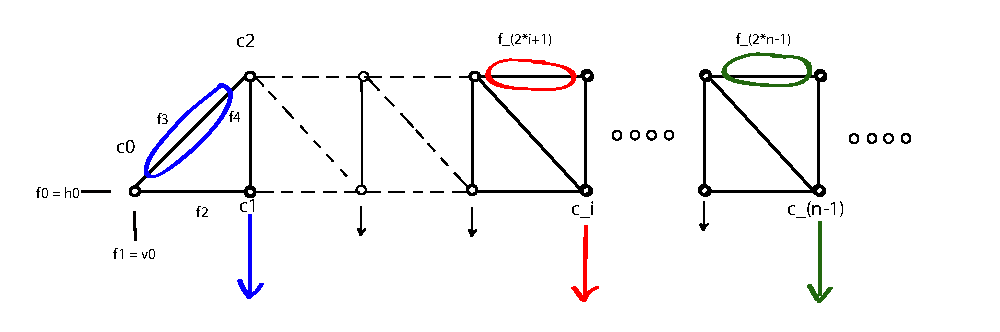
\includegraphics[keepaspectratio]{Imagenes/im_11.pdf}
		  \caption{Mayor carga aplicada sobre $c_{i} \Rightarrow$ fuerza de mayor módulo=$2*i+1$}
		  \label{fig:contra1}
	\end{center}
\end{figure}
\FloatBarrier

\subsubsection{Aumentando uniformemente el peso de todas las cargas}

En esta etapa de la experimentación aumentamos el peso de todas las cargas de igual manera. Para un determinado valor de $n$
fijamos $h=n$, $span=n$, y variamos el valor del peso de las cargas con valores entre 5 y 100 con saltos de 5 en 5. Los
resultados obtenidos fueron los siguientes:

\begin{figure}[!h]
	\begin{center}
		  \includegraphics[scale=0.4]{Imagenes/variable_cis/equal_cis/equal_cis_n_6}
		  \caption{Máximo módulo de las fuerzas en función del peso de las cargas para $n=6$}
		  \label{fig:contra1}
	\end{center}
\end{figure}
\FloatBarrier

\begin{figure}[!h]
	\begin{center}
		  \includegraphics[scale=0.4]{Imagenes/variable_cis/equal_cis/equal_cis_n_16}
		  \caption{Máximo módulo de las fuerzas en función del peso de las cargas para $n=16$}
		  \label{fig:contra1}
	\end{center}
\end{figure}
\FloatBarrier

\begin{figure}[!h]
	\begin{center}
		  \includegraphics[scale=0.4]{Imagenes/variable_cis/equal_cis/equal_cis_n_32}
		  \caption{Máximo módulo de las fuerzas en función del peso de las cargas para $n=32$}
		  \label{fig:contra1}
	\end{center}
\end{figure}

Nuevamente, parecería ser el aumento del máximo módulo entre todas las fuerzas es directamente proporcional al peso de
todas las cargas. Observemos que comparando el experimento anterior y este para los mismos valores de $n$, el 
máximo módulo cuando se aumenta el peso de todas las cargas es mucho mayor que cuando se aumenta el peso de solo una de
ellas.

\subsubsection{Aumentando únicamente el peso de la carga del medio}

Las condiciones de este último experimento son muy similares a las del anterior: Para un determinado $n$,
$span=n$, $h=n$. Sin embargo, en este caso el peso de las cargas = 1 para todas menos para la central.
Vamos variando este último entre 5 y 100, con saltos de 5 en 5

\begin{figure}[!h]
	\begin{center}
		  \includegraphics[scale=0.4]{Imagenes/variable_cis/just_middle_ci/just_middle_ci_n_6}
		  \caption{Máximo módulo de las fuerzas en función del peso de las carga del medio para $n=6$}
		  \label{fig:contra1}
	\end{center}
\end{figure}

\begin{figure}[!h]
	\begin{center}
		  \includegraphics[scale=0.4]{Imagenes/variable_cis/just_middle_ci/just_middle_ci_n_16}
		  \caption{Máximo módulo de las fuerzas en función del peso de las carga del medio para $n=16$}
		  \label{fig:contra1}
	\end{center}
\end{figure}

\begin{figure}[!h]
	\begin{center}
		  \includegraphics[scale=0.4]{Imagenes/variable_cis/just_middle_ci/just_middle_ci_n_32}
		  \caption{Máximo módulo de las fuerzas en función del peso de las carga del medio para $n=32$}
		  \label{fig:contra1}
	\end{center}
\end{figure}

Nuevamente observamos un aumento directamente proporcional entre ambas variables. Si bien no es posible verlo a partir de
los gráficos, también corroboramos la hipótesis planteada en el desarrollo respecto a la conservación de la
simetría de las fuerzas. Finalmente es necesario destacar que el aumento en el 
valor del máximo módulo para mismos valores de $n$ es mucho menor al del experimento anterior, en el que se aumentaba
el peso de todas las cargas.

~

\subsection{Heurística}

Efectivamente pudimos comprobar que la heurística propuesta funciona bien. Las ideas descriptas en el desarrollo se basan
en los resultados experimentales. El método fue probado para distintas instancias con
distintos valores de \emph{n} y distintas distribuciones de las cargas dando resultados coherentes.
Junto con el trabajo se incluye una carpeta llamada ''instancias'', que contiene archivos de prueba para probar el método.













\section{Conclusiones}

%	Los experimentos realizados demuestran que las magnitudes de las fuerzas aplicadas sobre los links de la estructura
varían en función del largo de la estructura, de la cantidad de secciones, del peso de las cargas y de la distribución
de las mismas (No es lo mismo concentrar gran parte del peso en el medio de la estructura, que sobre uno de los extremos,
o de manera uniforme). En particular las magnitudes aumentan para estructuras con un \emph{span} más largo y, lógicamente,
cuando se aplica más peso sobre la misma.

	La heurística constituye una buena solución a nuestro problema,
ya que se basa en los experimentos mencionados anteriormente. Intenta eliminar las cargas más pesadas (mayores en módulo)
reemplazándolas por pilares, y en el caso de que el peso esté uniformemente distribuído ubica un pilar en el medio,
reduciendo el \emph{span} de ambas subestructuras. Sin embargo hay casos en donde no puede generar un puente seguro,
pero ningún otro algoritmo podría. Por ejemplo, un puente de tan solo 2 secciones en donde la única carga aplicada
es demasiado pesada. (2 es la mínima cantidad de secciones de un puente ''Prat Truss'').

	Aplicar ''Eliminación Gaussiana'' para resolver un problema concreto de la vida real resultó motivante y de gran
interés. En suma, encontrar una buena representación de la matriz banda y luego adaptar el método fue un desafío
bastante grande.

	Finalmente podemos mencionar que la primera parte del trabajo, en donde planteamos el sistema e inicializamos
la matriz fue sin dudas la más difícil, ya que es un procedimiento que hicimos de forma casi ''manual'', y por lo
tanto encontrar
errores en esta parte del código resultó ser una tarea ardua y trabajosa.

\section{Apéndices}

%\input{apendices.tex}

\section{Referencias}

%\input{referencias.tex}

\end{document}
